% flowchart.tex — conceptual diagram of the estimation procedure (Figure 1). No equations; only the equation numbers in the text are cited.
%
%   Build: pdflatex flowchart.tex && pdfcrop --margins 3 flowchart.pdf figs/flowchart.pdf \
%          && pdftoppm -png -r 400 -singlefile figs/flowchart.pdf figs/flowchart && rm flowchart.pdf
%   Text is \footnotesize (8 pt) — the figure is about 180 mm wide, so it stays at or above 7 pt at double-column width. No grey text.
%   Colour by role only (Okabe-Ito): grey fill = input data · white = computation · green = calibration · blue = output.
\documentclass[border=3pt]{standalone}
\usepackage{amsmath,amssymb}
\usepackage{tikz}
\usetikzlibrary{arrows.meta,fit,backgrounds}
\definecolor{cOut}{HTML}{0072B2}
\definecolor{cCal}{HTML}{009E73}
\begin{document}
\sffamily\footnotesize
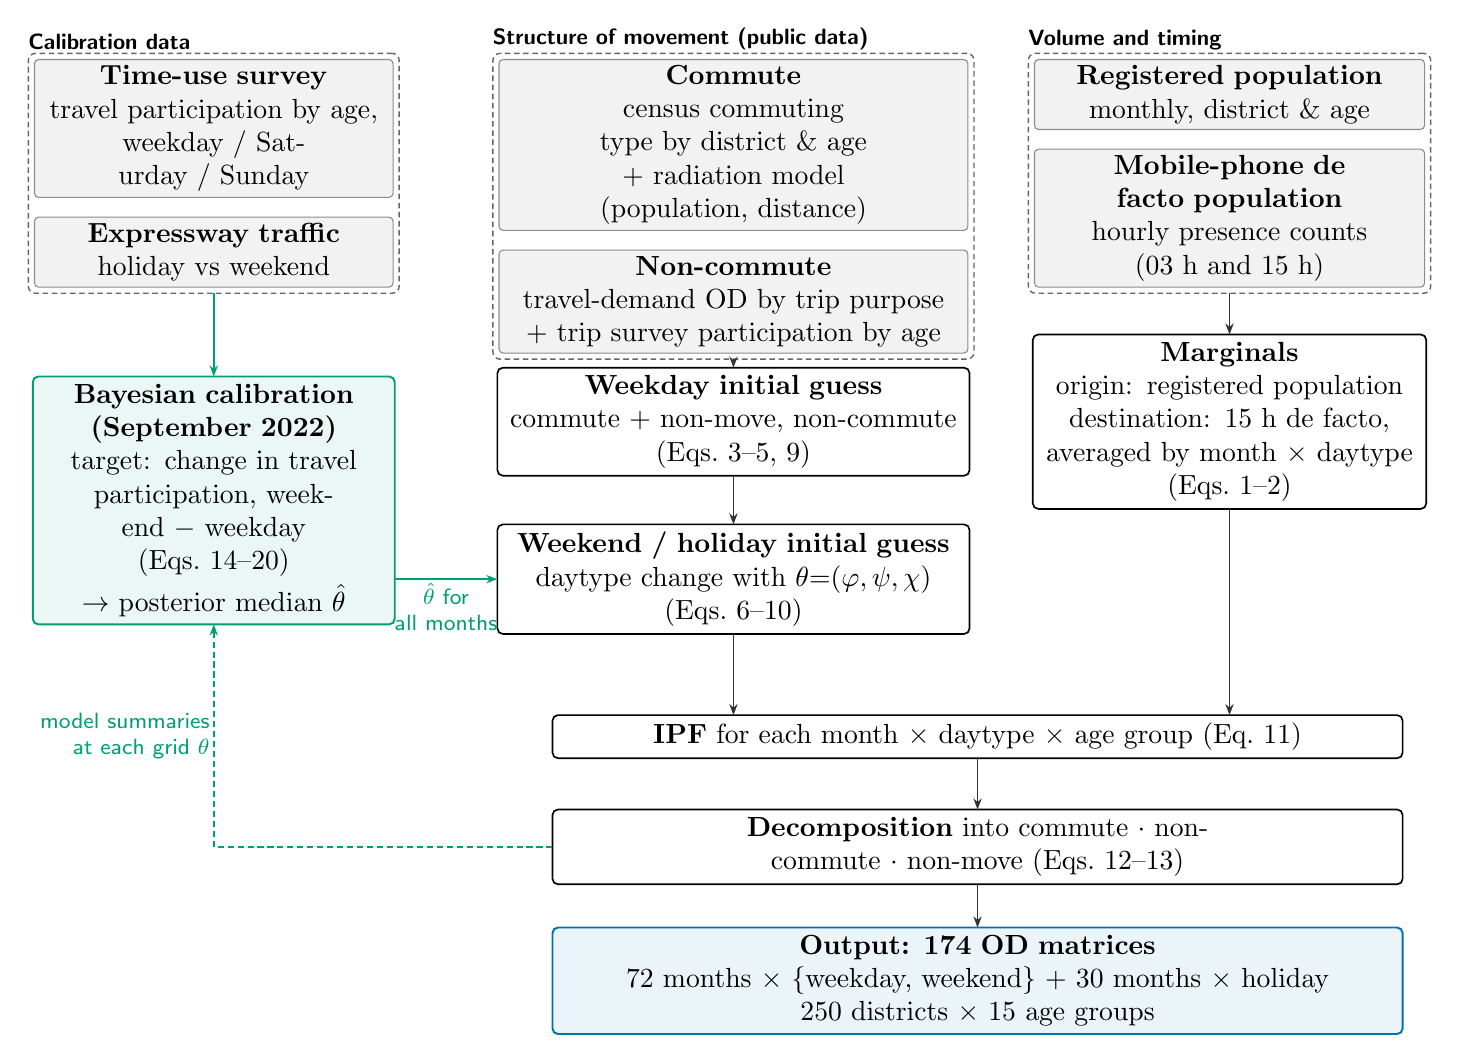
\begin{tikzpicture}[x=1mm, y=1mm,
    every node/.style={inner sep=0pt, outer sep=0pt},
    data/.style ={draw=black!45, fill=black!5, rounded corners=1.5pt, line width=.4pt,
                  align=center, inner sep=2.2pt},
    stage/.style={draw=black, fill=white, rounded corners=2pt, line width=.6pt,
                  align=center, inner sep=2.8pt},
    cal/.style  ={draw=cCal, fill=cCal!8, rounded corners=2pt, line width=.7pt,
                  align=center, inner sep=2.8pt},
    outb/.style ={draw=cOut, fill=cOut!8, rounded corners=2pt, line width=.7pt,
                  align=center, inner sep=2.8pt},
    grp/.style  ={draw=black!60, dash pattern=on 2pt off 1.3pt, rounded corners=2.5pt,
                  line width=.5pt, inner sep=2.2pt},
    hdr/.style  ={anchor=south west, font=\sffamily\footnotesize\bfseries},
    ar/.style   ={-{Stealth[length=4pt,width=3pt]}, draw=black!80, line width=.55pt},
    arc/.style  ={-{Stealth[length=4pt,width=3pt]}, draw=cCal, line width=.65pt},
    ard/.style  ={-{Stealth[length=4pt,width=3pt]}, draw=cCal, line width=.55pt,
                  dash pattern=on 2.2pt off 1.4pt}]

\def\LX{24}  \def\MX{90}  \def\RX{153}   % column centres
\def\LW{44}  \def\MW{58}  \def\RW{48}    % column widths (mm, text width)

% ── input data — three groups ──────────────────────────────────────────────
\node[data, text width=\LW mm, anchor=north] (tus) at (\LX,0)
  {\textbf{Time-use survey}\\travel participation by age,\\weekday / Saturday / Sunday};
\node[data, text width=\LW mm, anchor=north] (hw)  at ([yshift=-2.5mm]tus.south)
  {\textbf{Expressway traffic}\\holiday vs weekend};

\node[data, text width=\MW mm, anchor=north] (cin) at (\MX,0)
  {\textbf{Commute}\\census commuting type by district \& age\\+ radiation model (population, distance)};
\node[data, text width=\MW mm, anchor=north] (nin) at ([yshift=-2.5mm]cin.south)
  {\textbf{Non-commute}\\travel-demand OD by trip purpose\\+ trip survey participation by age};

\node[data, text width=\RW mm, anchor=north] (reg) at (\RX,0)
  {\textbf{Registered population}\\monthly, district \& age};
\node[data, text width=\RW mm, anchor=north] (dfp) at ([yshift=-2.5mm]reg.south)
  {\textbf{Mobile-phone de facto population}\\hourly presence counts\\(03 h and 15 h)};

\begin{scope}[on background layer]
  \node[grp, fit=(tus)(hw)] (gL) {};
  \node[grp, fit=(cin)(nin)] (gM) {};
  \node[grp, fit=(reg)(dfp)] (gR) {};
\end{scope}
\node[hdr] at ([yshift=1.3pt]gL.north west) {Calibration data};
\node[hdr] at ([yshift=1.3pt]gM.north west) {Structure of movement (public data)};
\node[hdr] at ([yshift=1.3pt]gR.north west) {Volume and timing};

% ── computation ─────────────────────────────────────────────────────────
\node[stage, text width=\MW mm] (wk) at (\MX,-46)
  {\textbf{Weekday initial guess}\\commute + non-move, non-commute\\(Eqs.~3--5, 9)};
\node[stage, text width=\RW mm] (mg) at (\RX,-46)
  {\textbf{Marginals}\\origin: registered population\\destination: 15 h de facto,\\averaged by month $\times$ daytype\\(Eqs.~1--2)};
\node[stage, text width=\MW mm] (dt) at (\MX,-66)
  {\textbf{Weekend / holiday initial guess}\\daytype change with $\theta{=}(\varphi,\psi,\chi)$\\(Eqs.~6--10)};
\node[cal, text width=\LW mm] (cb) at (\LX,-56)
  {\textbf{Bayesian calibration}\\\textbf{(September 2022)}\\target: change in travel\\participation, weekend $-$ weekday\\(Eqs.~14--20)\\[2pt]
   $\rightarrow$ posterior median $\hat\theta$};

\node[stage, text width=106mm] (ipf) at (121,-86)
  {\textbf{IPF} for each month $\times$ daytype $\times$ age group (Eq.~11)};
\node[stage, text width=106mm] (sp) at (121,-100)
  {\textbf{Decomposition} into commute $\cdot$ non-commute $\cdot$ non-move (Eqs.~12--13)};
\node[outb, text width=106mm] (o) at (121,-117)
  {\textbf{Output: 174 OD matrices}\\72 months $\times$ \{weekday, weekend\} + 30 months $\times$ holiday\\250 districts $\times$ 15 age groups};

% ── arrows ──────────────────────────────────────────────────────────────
\draw[arc] (gL.south) -- (cb.north);
\draw[ar]  (gM.south) -- (wk.north);
\draw[ar]  (gR.south) -- (mg.north);
\draw[ar]  (wk.south) -- (dt.north);
\draw[arc] (cb.east |- dt.west) -- node[below, font=\sffamily\footnotesize, text=cCal, yshift=-1.5pt, align=center]
  {$\hat\theta$ for\\all months} (dt.west);
\draw[ar]  (dt.south) -- (dt.south |- ipf.north);
\draw[ar]  (mg.south) -- (mg.south |- ipf.north);
\draw[ar]  (ipf.south) -- (sp.north);
\draw[ar]  (sp.south) -- (o.north);
% calibration solves IPF · decomposition for each grid θ in September 2022 to obtain model values
\draw[ard] (sp.west) -- (\LX,-100) -- node[left, font=\sffamily\footnotesize, text=cCal, xshift=-1.5pt, align=right]
  {model summaries\\at each grid $\theta$} (cb.south);
\end{tikzpicture}
\end{document}
